
%% bare_conf.tex
%% V1.4b
%% 2015/08/26
%% by Michael Shell
%% See:
%% http://www.michaelshell.org/
%% for current contact information.
%%
%% This is a skeleton file demonstrating the use of IEEEtran.cls
%% (requires IEEEtran.cls version 1.8b or later) with an IEEE
%% conference paper.
%%
%% Support sites:
%% http://www.michaelshell.org/tex/ieeetran/
%% http://www.ctan.org/pkg/ieeetran
%% and
%% http://www.ieee.org/

%%*************************************************************************
%% Legal Notice:
%% This code is offered as-is without any warranty either expressed or
%% implied; without even the implied warranty of MERCHANTABILITY or
%% FITNESS FOR A PARTICULAR PURPOSE! 
%% User assumes all risk.
%% In no event shall the IEEE or any contributor to this code be liable for
%% any damages or losses, including, but not limited to, incidental,
%% consequential, or any other damages, resulting from the use or misuse
%% of any information contained here.
%%
%% All comments are the opinions of their respective authors and are not
%% necessarily endorsed by the IEEE.
%%
%% This work is distributed under the LaTeX Project Public License (LPPL)
%% ( http://www.latex-project.org/ ) version 1.3, and may be freely used,
%% distributed and modified. A copy of the LPPL, version 1.3, is included
%% in the base LaTeX documentation of all distributions of LaTeX released
%% 2003/12/01 or later.
%% Retain all contribution notices and credits.
%% ** Modified files should be clearly indicated as such, including  **
%% ** renaming them and changing author support contact information. **
%%*************************************************************************


% *** Authors should verify (and, if needed, correct) their LaTeX system  ***
% *** with the testflow diagnostic prior to trusting their LaTeX platform ***
% *** with production work. The IEEE's font choices and paper sizes can   ***
% *** trigger bugs that do not appear when using other class files.       ***                          ***
% The testflow support page is at:
% http://www.michaelshell.org/tex/testflow/



\documentclass[11pt]{IEEEtran}
% Some Computer Society conferences also require the compsoc mode option,
% but others use the standard conference format.
% If IEEEtran.cls has not been installed into the LaTeX system files,
% manually specify the path to it like:
% \documentclass[conference]{../sty/IEEEtran}





% Some very useful LaTeX packages include:
% (uncomment the ones you want to load)


% *** MISC UTILITY PACKAGES ***
%
%\usepackage{ifpdf}
% Heiko Oberdiek's ifpdf.sty is very useful if you need conditional
% compilation based on whether the output is pdf or dvi.
% usage:
% \ifpdf
%   % pdf code
% \else
%   % dvi code
% \fi
% The latest version of ifpdf.sty can be obtained from:
% http://www.ctan.org/pkg/ifpdf
% Also, note that IEEEtran.cls V1.7 and later provides a builtin
% \ifCLASSINFOpdf conditional that works the same way.
% When switching from latex to pdflatex and vice-versa, the compiler may
% have to be run twice to clear warning/error messages.
\usepackage{graphicx}
\usepackage[justification=centering]{caption}





% *** CITATION PACKAGES ***
%
%\usepackage{cite}
% cite.sty was written by Donald Arseneau
% V1.6 and later of IEEEtran pre-defines the format of the cite.sty package
% \cite{} output to follow that of the IEEE. Loading the cite package will
% result in citation numbers being automatically sorted and properly
% "compressed/ranged". e.g., [1], [9], [2], [7], [5], [6] without using
% cite.sty will become [1], [2], [5]--[7], [9] using cite.sty. cite.sty's
% \cite will automatically add leading space, if needed. Use cite.sty's
% noadjust option (cite.sty V3.8 and later) if you want to turn this off
% such as if a citation ever needs to be enclosed in parenthesis.
% cite.sty is already installed on most LaTeX systems. Be sure and use
% version 5.0 (2009-03-20) and later if using hyperref.sty.
% The latest version can be obtained at:
% http://www.ctan.org/pkg/cite
% The documentation is contained in the cite.sty file itself.






% *** GRAPHICS RELATED PACKAGES ***
%
\ifCLASSINFOpdf
  % \usepackage[pdftex]{graphicx}
  % declare the path(s) where your graphic files are
  % \graphicspath{{../pdf/}{../jpeg/}}
  % and their extensions so you won't have to specify these with
  % every instance of \includegraphics
  % \DeclareGraphicsExtensions{.pdf,.jpeg,.png}
\else
  % or other class option (dvipsone, dvipdf, if not using dvips). graphicx
  % will default to the driver specified in the system graphics.cfg if no
  % driver is specified.
  % \usepackage[dvips]{graphicx}
  % declare the path(s) where your graphic files are
  % \graphicspath{{../eps/}}
  % and their extensions so you won't have to specify these with
  % every instance of \includegraphics
  % \DeclareGraphicsExtensions{.eps}
\fi


% correct bad hyphenation here
\hyphenation{op-tical net-works semi-conduc-tor}


\begin{document}
%
% paper title
% Titles are generally capitalized except for words such as a, an, and, as,
% at, but, by, for, in, nor, of, on, or, the, to and up, which are usually
% not capitalized unless they are the first or last word of the title.
% Linebreaks \\ can be used within to get better formatting as desired.
% Do not put math or special symbols in the title.
\title{Characterizing Sub-THz Curving Beams with Modified Gerchberg-Saxton Phase Retrieval Algorithms }


% author names and affiliations
% use a multiple column layout for up to three different
% affiliations
\author{\IEEEauthorblockN{Alan Chavez\\}
\IEEEauthorblockA{Rice University
}}

\maketitle


\IEEEpeerreviewmaketitle

\section{Introduction}

Curving beams have recently drawn significant interest in academia due to their unique potential to mitigate blocking events in communications and sensing applications.
In prior literature, the trajectory of such beams has been determined through two-dimensional spatial heatmaps of measured intensity\cite{AiryObservation, spindel_ms}.
Although effective, this approach is impractical in real world settings where complete spatial field measurements are unavailable or infeasible.
This limitation is particularly meaningful in sensing and jamming scenarios, where a fast and accurate determination of a beam's path is critical for performance.

Previous works on the trajectory of curving beams have shown that Airy beams, as well as arbitrary caustic beams encode the trajectory of the beam into it's transmit aperture\cite{AiryObservation, Froehly}.
Airy beams encode their trajectory by modifying both the amplitude and phase of the electric field at the aperture\cite{AiryObservation}, however caustic beams, and other common beams such as beam deflections, and Bessel beams only require modulation of the phase profile at the aperture\cite{Froehly, beam_tutorial}.
This observation implies that reconstructing the phase profile at the transmit aperture could enable prediction of the beam's curved path without the need for exhaustive heatmap measurements.

To the best of my knowledge, prior work has not explored if it is possible to retrieve the phase imposed by the transmit aperture for a bending beam. 
In this work, I investigate the use of an iterative phase retrieval algorithm to retrieve the phase profile at the transmit aperture from one dimensional measurements.
The recovered phase profile is then decoded, and used to compute the curving beam's trajectory.

\section{Iterative Phase retrieval}

The Gerchberg--Saxton (GS) algorithm is an iterative phase retrieval method that reconstructs a complex wavefront from intensity measurements in two related planes which are hence referred to as the transmit aperture and receive aperture.
Starting with an initial guess for the phase, the algorithm propagates the wavefront forward and backward between the two measurement planes while constraining the amplitude in each plane with measured values\cite{generic_mgs}.
The phase of the wavefront is left unconstrained which causes small changes towards a solution each propagation.
After some amount of iterations the algorithm converges on a solution, which is not guaranteed to be unique\cite{generic_mgs}.
GS is widely used in optical frequencies for imaging, and holography, however it requires multiple modifications to function effectively in the sub-THz regime.

The first required modification is to replace the use of a Fraunhofer diffraction as a model for wavefront propagation with Rayleigh-Sommerfeld\cite{mmwave_phase_retrieval}.
Although the Fraunhofer diffraction model is pragmatic in optics, in the sub-THz regime meaningful measurements of curving beams take place in the near-field region.
The change in propagation model increases the computational complexity from 1 Fast Fourier Transforms (FFT) per propagation, to 3 FFTs, however it is necessary to achieve accuracy in the near-field\cite{rs_impl}.

Despite the improved propagation model, GS frequently does not converge, and when it does converge, it converges on a low quality result.
To further improve the quality of the results a second modification is made to introduce gradient descent, which has been shown to improve the quality of results at optical frequencies\cite{mgs_descent}.
Instead of letting the phase remain unconstrained during iterations, a weighted mean square error (MSE) is computed in the receive aperture plane.
The error is weighted to favor the higher amplitude sections of the measured data where the signal-to-noise ratio (SNR) is highest.
The MSE is then propagated back to the transmit plane where a gradient is computed.
The transmit aperture phase is modified to decrease the weighted MSE and then forward propagated to the receive plane for the next iteration, as described in Sec.~3 of Liu and Takaki~\cite{mgs_descent}.
To further improve the quality of results, phase measurements are required at the receive aperture.
Although phase cannot be easily measured at optical frequencies, only intensity, it is pragmatic and beneficial to measure amplitude and phase in the sub-THz regime.


\section{Inverting the Froehly Equation}

The Froehly equation maps an arbitrary curved beam trajectory to the phase profile needed at the transmit aperture\cite{Froehly}.
To characterize a curving beam the opposite functionality is needed: given a phase profile, compute a beam's trajectory.
It is unlikely that a unique analytic inverse solution exists for all phase profiles since there are multiple different trajectories that can be hard to distinguish from each other without further knowledge.
However multiple numerical solutions exist, such as an error optimization approach or a brute force approach.
The computation cost of a brute force approach is negligible compared to the phase retrieval stage, convenient to implement, and embarrassingly parallel.
Therefore I adopted the brute force approach.
In this approach a set of parameters is exhaustively swept to create a set of candidate trajectories.
Each candidate trajectory is used to compute a phase profile, which is then compared against the phase profile measured by the prior phase retrieval stage.
The candidate trajectory that produces the lowest MSE is selected as the real trajectory.

\section{Simulation Results}

To test the accuracy of the proposed new method, the phase retrieval stage and trajectory computation stages are first tested independently and then together.

\subsection{Phase Retrieval Simulation Results}

To simulate the effectiveness of the proposed phase retrieval algorithm a trajectory, transmit aperture, and receive aperture are chosen.
The specific values of the trajectories, and apertures are chosen to mimic what the Rice Networks Group's KeySight testbed can reasonably accomplish.
Transmit apertures are kept roughly near 100 mm wide, and receive aperture are between 300 and 100 mm wide.
The receive aperture is placed on the propagation axis between 100 and 300 mm away from the transmit aperture.
The concavity of the curve is kept relatively shallow.
The trajectory is modeled as the polynomial Eq. ~\ref{eq:quadratic trajectory} where The coefficients are restricted to the ranges \(A, B \in [-0.5, 0.5]\) and \(C \in [-0.1, 0.1]\) to match the testbed's capabilities.

\begin{equation}
A x^2 + B x + C
\label{eq:quadratic trajectory}
\end{equation}

Figures \ref{fig:good_qual_orig}, \ref{fig:good_qual_rec}, and \ref{fig:good_qual_phase} show simulation results for a well conditioned scenario that converges on the correct phase profile.
The scenario is well conditioned due to the fact that the receive aperture captures the entire beam, and has measurements spread approximately 0.01 mm apart or \(\lambda\)/20.0.
In this particular simulation the phase retrieval algorithm converged after 3200 iterations and had weighted MSE of \(8 \cdot 10^{-5}\).

Various conditions can cause the quality of results as measured by weighted MSE to worsen dramatically.
If the receive aperture does not capture the main lobe and side lobes of the beam, then the algorithm will either fail to converge or converge with an error greater than 0.05, which cannot produce an accurate trajectory computation.
Furthermore, as the density of measurements is lowered the error rises quickly.
Although, this is not explored quantitatively, it appears that a density of measurement less that \(\lambda\) will not produce usable results.

\begin{figure}[]
    \centering
    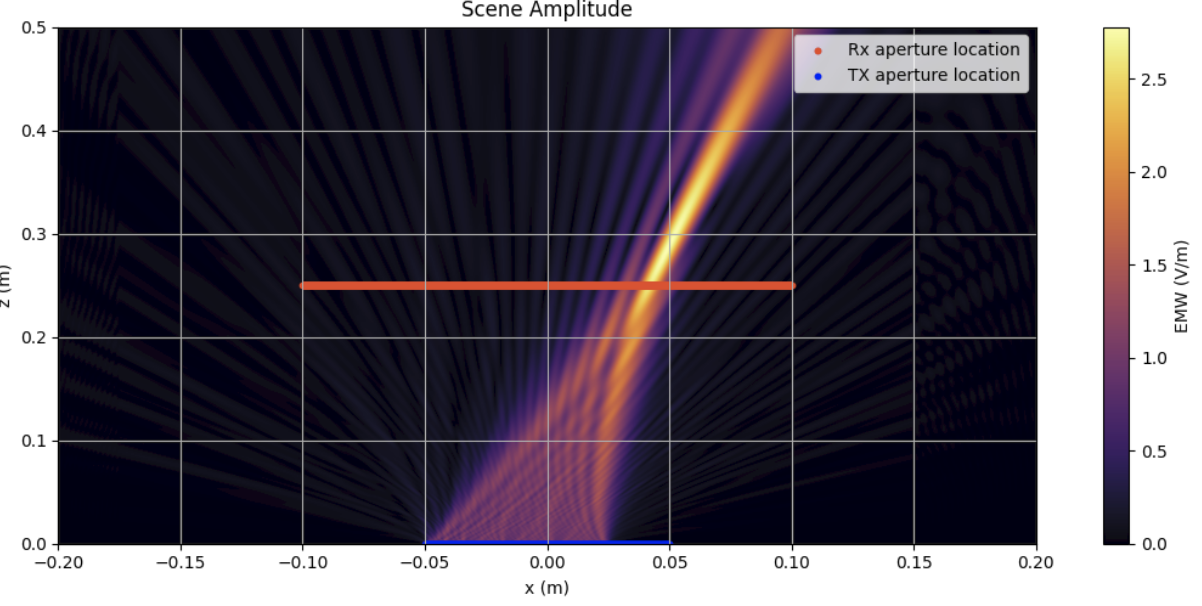
\includegraphics[width=1.0\linewidth]{good_qual_orig.png}
    \caption{Well Conditioned Simulation Original}
    \label{fig:good_qual_orig}
\end{figure}

\begin{figure}[]
    \centering
    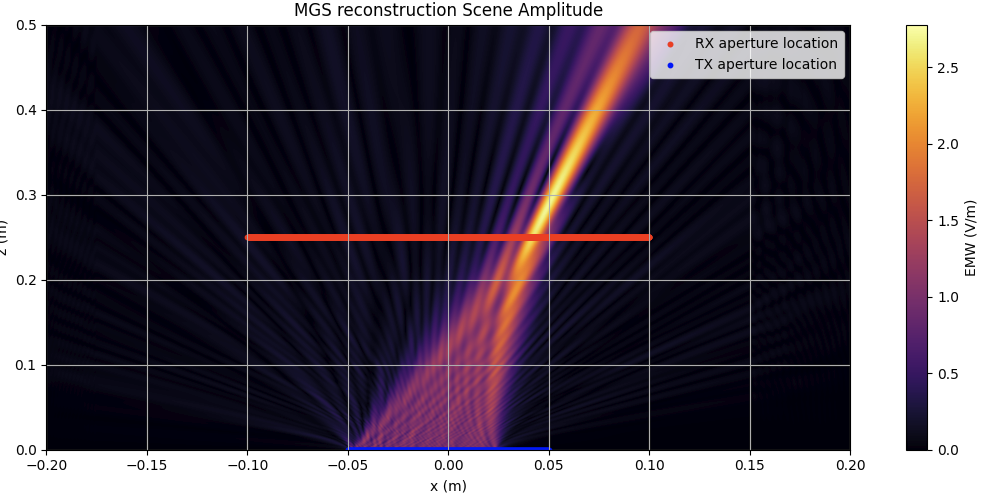
\includegraphics[width=1.0\linewidth]{good_qual_rec.png}
    \caption{Well Conditioned Simulation Reconstructed}
    \label{fig:good_qual_rec}
\end{figure}

\begin{figure}[]
    \centering
    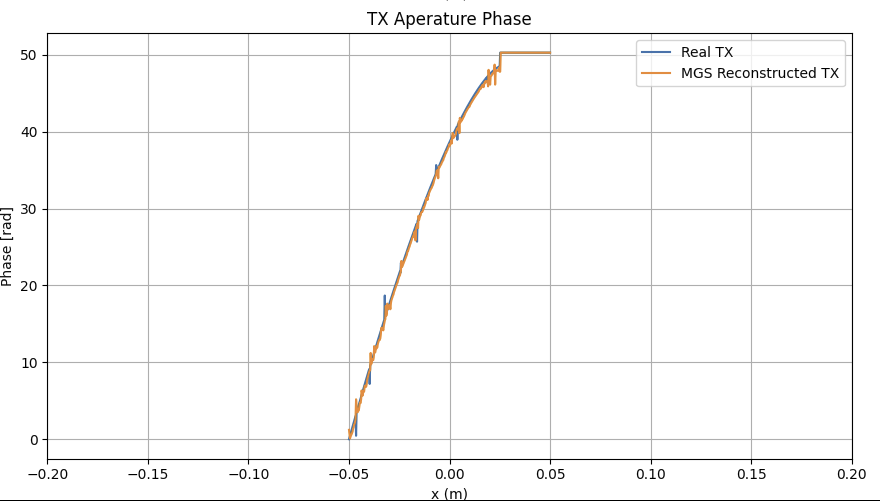
\includegraphics[width=1.0 \linewidth]{good_qual_phase.png}
    \caption{Well Conditioned Simulation Phase Profile Comparison}
    \label{fig:good_qual_phase}
\end{figure}

\subsection{Trajectory Computation Simulation Results}

Figure \ref{fig:good_qual_traj} shows the recovered trajectory versus the real trajectory of the beam when closely spaced receive measurements are used.
Although the recovered trajectory in this case has an MSE of roughly 0.126 at the transmit aperture, the trajectories are nearly identical.
This shows that while the phase retrieval method is not perfect, it does provide enough information to accurately predict the trajectory.
Figure \ref{fig:bad_condition_traj.png} shows the recovered trajectory of a beam when receive measurements were spaced too far apart to support an accurate phase retrieval.
This results in the recovered trajectory being wrong by roughly 25mm at the the transmit aperture.
It is worth noting that the recovered trajectory seems to become more accurate as the propagation distance increases.

\begin{figure}[]
    \centering
    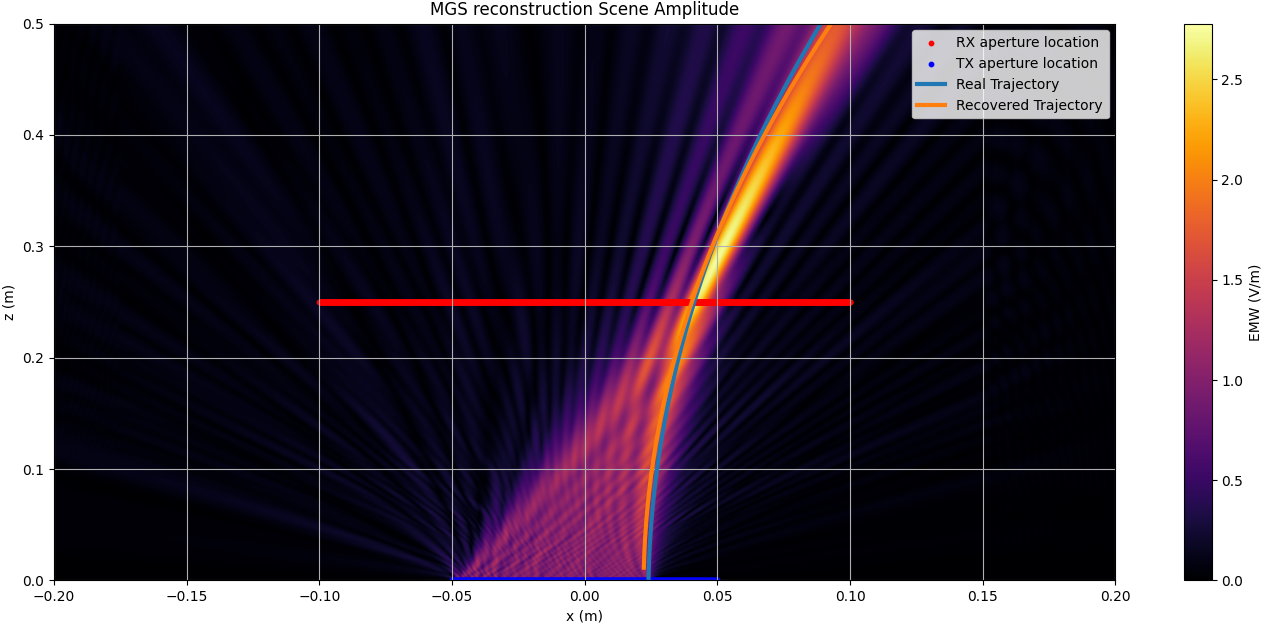
\includegraphics[width=1.0\linewidth]{good_qual_traj.png}
    \caption{Trajectory Reconstruction \(\lambda\)/20 Spacing}
    \label{fig:good_qual_traj}
\end{figure}

\begin{figure}[]
    \centering
    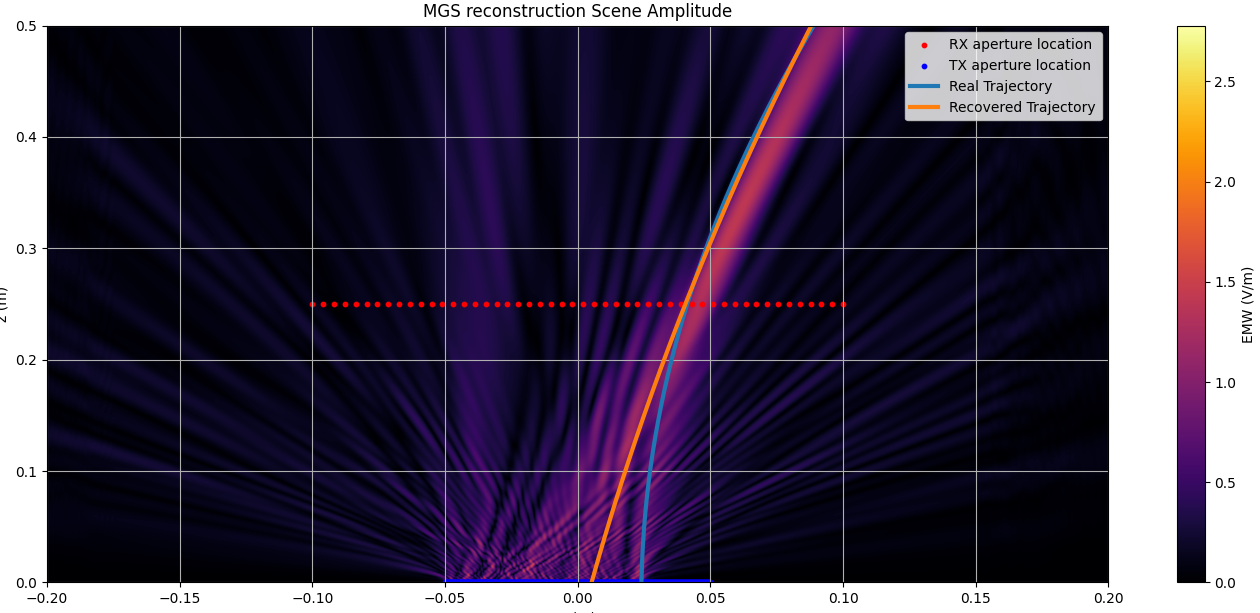
\includegraphics[width=1.0 \linewidth]{bad_condition_traj.png}
    \caption{Trajectory Reconstruction 2\(\lambda\) Spacing}
    \label{fig:bad_condition_traj.png}
\end{figure}



\section{Limitations of Proposed Approach}

One of the limitations of the proposed approach for characterizing curving beams is the extraordinary computation cost for even well conditioned scenarios.
The amount of iterations frequently exceeds 3000, with each iteration containing upwards of 30 FFTs computed.
Furthermore, the phase retrieval algorithm is not guaranteed to converge on the correct results, converge at all, or converge with a deterministic amount of time.
These computation limits will can cause this approach to be infeasible for real time systems requiring results within a second, or embedded systems with limited compute resources.

Furthermore, the phase retrieval approach requires dense measurements that can take a prohibitive amount of time when using a synthetic aperture receiver.
The benefits of only requiring one dimension of measurement may be counteracted by the increased amount of time it takes to gather precise data.

To successfully use the proposed phase retrieval algorithm requires knowledge about the scenario that may not be practical.
The receiver must be capable of accurately measuring phase.
Measuring phase information can be practical in a sensing application where the synchronization between the transmitter and receiver can be guaranteed, however in adversarial situations it may be more difficult to accurately measure phase.

Lastly, the proposed method requires knowledge of the aperture of the transmitter, since solutions to the phase retrieval algorithm are not guaranteed to be unique, without knowledge of the transmitter's aperture size, it can be impossible to characterize the trajectory accurately.

\section{Conclusion}

This work demonstrated a methodology for characterizing sub-THz curving beams by combining a modified Gerchberg--Saxton phase retrieval algorithm with a brute-force inversion of the Froehly equation.
The modified GS approach, incorporating Rayleigh-Sommerfeld propagation and gradient descent MSE optimization updates, was shown in simulation to reconstruct accurate aperture phase profiles under well-conditioned measurement scenarios.
By matching the retrieved phase profiles against a set of trajectory candidates, the beam trajectory could be estimated without requiring exhaustive two dimensional heatmap measurements.

Simulation results confirmed that accurate trajectory recovery is possible when the receive aperture fully captures the beam’s energy and the measurement sampling is sufficiently dense.
However, the proposed method’s high computational cost, sensitivity to measurement conditions, and reliance on receivers that are phase capable can limit the usefulness of the proposed solution for real time and resource-constrained systems.
Despite these challenges, the proposed approach offers a promising pathway toward efficient characterization of complex beam trajectories in scenarios where conventional field-mapping techniques are impractical.
Future work will focus on experimental validation, and quantitative analysis of the limits of the proposed system.



% conference papers do not normally have an appendix


% trigger a \newpage just before the given reference
% number - used to balance the columns on the last page
% adjust value as needed - may need to be readjusted if
% the document is modified later
%\IEEEtriggeratref{8}
% The "triggered" command can be changed if desired:
%\IEEEtriggercmd{\enlargethispage{-5in}}

% references section

% can use a bibliography generated by BibTeX as a .bbl file
% BibTeX documentation can be easily obtained at:
% http://mirror.ctan.org/biblio/bibtex/contrib/doc/
% The IEEEtran BibTeX style support page is at:
% http://www.michaelshell.org/tex/ieeetran/bibtex/
%\bibliographystyle{IEEEtran}
% argument is your BibTeX string definitions and bibliography database(s)
%\bibliography{IEEEabrv,../bib/paper}
%
% <OR> manually copy in the resultant .bbl file
% set second argument of \begin to the number of references
% (used to reserve space for the reference number labels box)
\bibliographystyle{plain}
\bibliography{main}



% that's all folks
\end{document}


